\documentclass{article}

\usepackage{latexsym}
\usepackage{fancyhdr}
\usepackage{amsmath}
\usepackage{hyperref}
\usepackage{listings}
\usepackage{pdfpages}
\usepackage[margin=1.2in]{geometry}
\lhead{Charles Pehlivanian}
\chead{October 15, 2016}
\rhead{Implied Engine Documentation [Brief]}
\cfoot{\thepage}
\pagestyle{fancy}

\hypersetup{colorlinks=true, urlcolor=blue}

\begin{document}

\title{Implied Future Pricing Engine}
\author{Charles Pehlivanian}

\maketitle

\begin{abstract}

An algorithm is presented for the computation of implied quotes in a hypothetical market closely resembling CME WTI Crude (CL) futures, ICE/IPE Brent futures (B), or any one of the US crude product markets. The algorithm produces a full set of implied quote prices and sizes using only user-entered quote information. The algorithm is modular, and each leg quote (size, price) can be computed on its own execution thread. We exploit this structure to test a cpu-distributed version, using a consumer-producer queue with worker tasks consuming a user quote and generating multiple downstream implied quotes per input. 
\end{abstract}

\section*{Overview}
The major futures exchanges (CMEGroup, ICE, LIFFE, EUREX) depend on an underlying implied quote calculation to give the appearance of increased liquidity and narrowed spreads in their markets. This is done by disseminating, in addition to the user-entered quotes in each market, an additional set of implied quotes. Each implied quote is linked to two to many underlying user-entered quotes, and executing against an implied quote will ''unravel'' the chain and produce trades in all the underlying markets.  All participants face the exchange, and will receive their respective fills as if the initiating order occured in their market.

For example, at a a given point in time the user-entered bbo quotes in the SP EMini markets ESU6, ESZ6 may look like Table 1. The ESU6-ESZ6 roll market may also be active, and a purchase in this market results in a purchase of ESZ6, the December contract, and a sale of ESU6. In this case, the quotes given in Table 2. will appear in the roll market {\it regardless of whether there are any user-entered quotes there}. So there will at least be a bbo, if there are bbos in the respective outright markets. 


It is important to note that in all cases {\it the purchase of the roll is price-improved to the best implied quote price}. Furthermore, in many exchange matching models, the best implied quote is not part of the market feed, or the additional implied-quote feed is served on a delayed channel, and this price-improvement is invisible to the trader until the trade report occurs. For this and the following reasons, a client-side calculation of the full set of implied prices is beneficial:

\begin{itemize}
\item Implied quote generation can be don client-side faster than the exchange feed;
\item In some markets, implied prices are not published at all;
\item One can use a larger set of inputs to generate a more accurate fair value for a security;
\item One can base a faster signal generation framework on an efficient implied quote server.
\end{itemize}

We will present a high-level summary only of an algorithm for complete computation of implied quotes.

\clearpage
\begin{table}
\centering
\begin{tabular}{|l|c|c|c|c|c|}
\hline
Market & BidSize & BidPrice & AskPrice & AskSize\\
\hline
ESU6 & 566 & 2177.25 & 2177.50 & 766 \\
ESZ6 & 144 & 2176.50 & 2177.25 & 44 \\
\hline
\end{tabular}
\caption{User-entered Quotes}
\label{tab:template}
\end{table}

\begin{table}
\centering
\begin{tabular}{|l|c|c|c|c|c|}
\hline
Market & Impl. BidSize & Impl. BidPrice & Impl. AskPrice & Impl. AskSize\\
\hline
ESU6-ESZ6 & -144 & -1.00   & 0.00  & 44 \\
\hline
\end{tabular}
\caption{Implied Roll Quotes}
\label{tab:template}
\end{table}


\section*{Workflow}
A high-level workflow is presented. The application subscribes to the user-only (non-implied) quote feed (often on a faster channel than full implied feeds from the exchange, if those are available)  for the respective exchange. In this case, a simple market consisting of two outrights $O_1$, $O_2$, and one calendar spread $S_12$ is considered. The market feed is demultiplexed to 3 channels, one for each instrument. The price, size are passed through to a user-quote object, and also to each implied outright computation (1 for each leg only). The results of those computations are fed to the respective implied quote objects, and the user may query the synchronous merged (best of user and implied quote) for each outright market. Of course the graph is significantly more complicated for the typical case of 12 or more outrights, with associated calendar spreads.

\clearpage
\begin{figure}
\centering
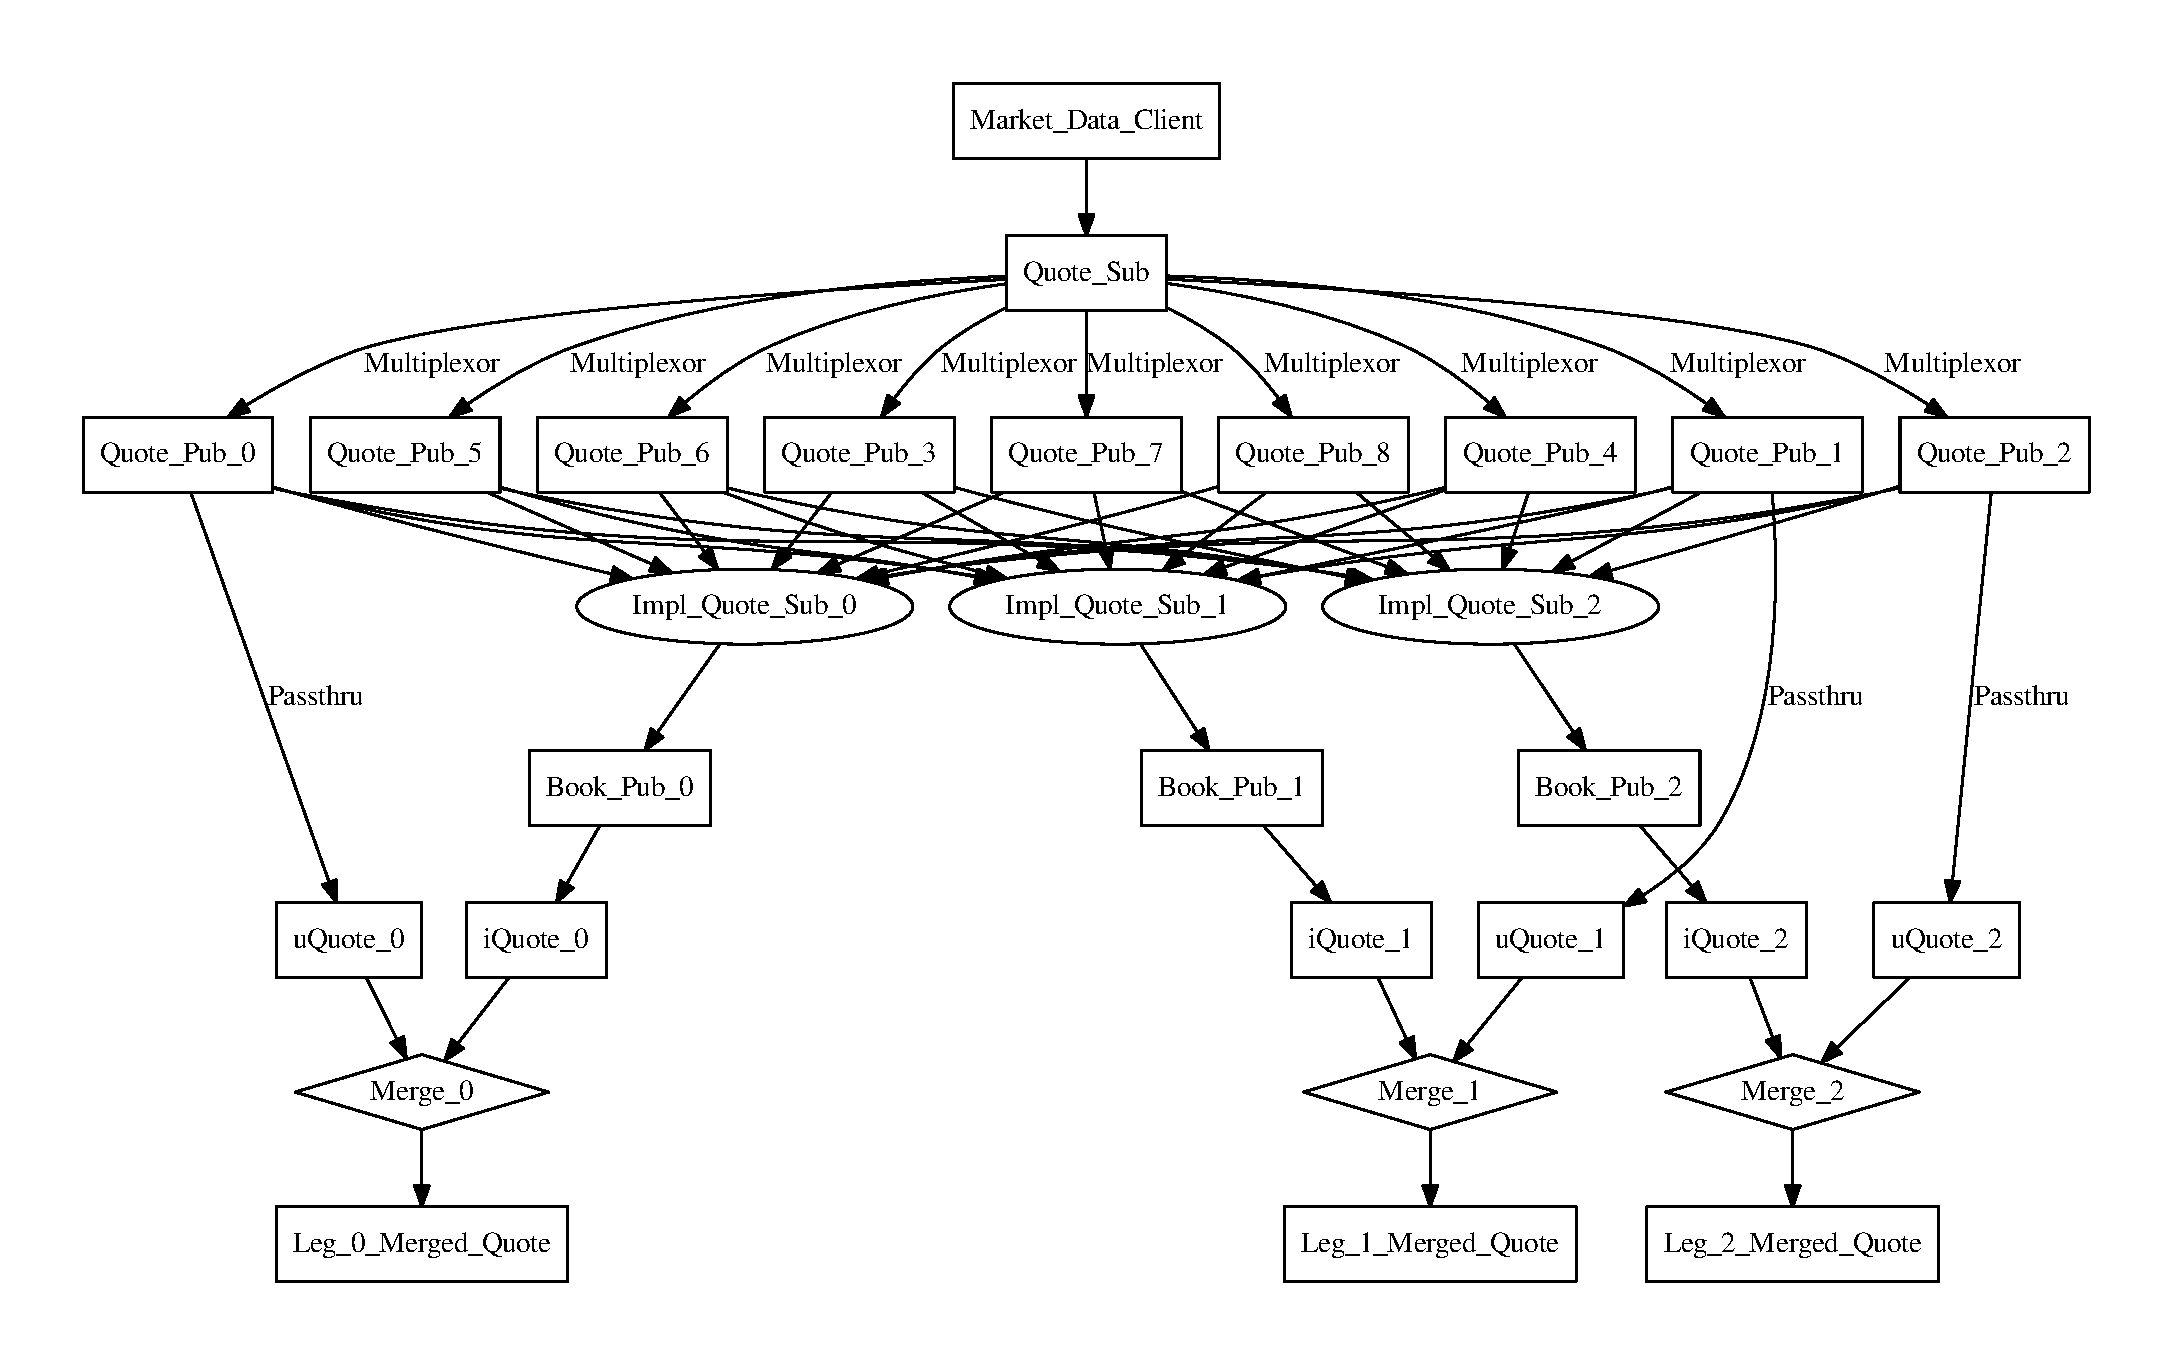
\includegraphics[scale=.44]{workflow.pdf}
\caption{High-level Workflow: 2 Outright Markets, 1 Calendar Spread}
\end{figure}

Notes
\begin{enumerate}
\item The initial demultiplexor separates the flow of 2 leg and 1 spread product and forwards them to one of 3 quote publishers.
\item The main algorithm and most of the work is performed in the oval nodes. Here multple leg, calendar spread quotes are consumed and an implied quote (price,size) is computed for the specified leg. There are 2 Calc nodes in this case. Care must be taken to ensure that these passes are threadsafe, and that the downstream merging is synchronized.
\item Separate user and implied quote objects (uQuote, iQuote) are maintained, and best-of or merged quotes are computed, and pushed to the client..
\end{enumerate}

\section*{Implementation}
The main entry point is the ImpliedServer$<$N$>$ class template, consisting of 2 components: a Client object for reading of quote information via socket, an ImpliedEngine$<$N$>$ object which is the computation engine, and a threadpool object for asynchronous calculations off of the main calc thread. Appropriate serialization and barriers are implemented within the ImpliedEngine$<$N$>$ class to ensure thread safety. The interface can be found on \href{https://github.com/pehlivanian/Implied_Price_Engine}{\it https://github.com/pehlivanian/Implied{\_}Price{\_}Engine/}

\begin{verbatim}

template<int N>
class ImpliedServer
{
public:
    ImpliedServer(bool sim_mode=true) :
            p_(std::make_unique<impl<ImpliedServer<N>>>(sim_mode)) { init_(); }
    void process() { preload_tasks_(); profiled_process_tasks_(); };

    // ...

private:
    void preload_tasks_();
    void process_tasks_();

    void init_();
    std::unique_ptr<impl<ImpliedServer>> p_;
};

template<int N>
struct impl<ImpliedServer<N>>
{
    impl(bool sim_mode) :
            sim_mode_(sim_mode),
            IE_(std::make_unique<ImpliedEngine<N>>()),
            C_(std::make_unique<Client>(8008, (char*)"0.0.0.0"))
           {}

    bool sim_mode_;
    std::unique_ptr<ImpliedEngine<N>> IE_;
    std::unique_ptr<Client> C_;

};

\end{verbatim}

We use the Eigen library for our linear algebra engine, and custom data structures, custom allocators, fast forward{\_}list, fast binary heap, fast customized  graph search/traversal algorithms for efficiency.

Within the ImpliedEngine<N> class, the main calculation algorithm makes use of some notions from linear algebra and graph theory. A typical graph for a 12-leg problem is shown in Figure 2., without expanation.

\begin{figure}
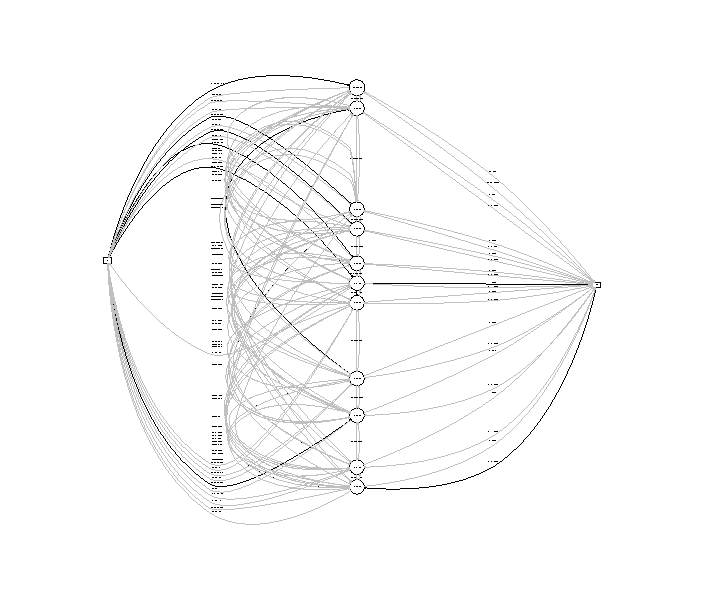
\includegraphics[scale=1.25]{test_case.pdf}
\caption{Setup for 12-leg Problem}
\end{figure}
\section*{Benchmarks}

The theoretical complexity of the algorithm is $O(n^2 log(n))$, where $n$ is the number of legs to calculate. I don't believe we can do any better than this, for theoretical reasons, unless we constrain the problem based on ad-hoc market structure considerations (no liquidity in certain markets, so we eliminate them from the calculation, etc.). In any case, the algorithm is highly configurable and will allow for most such constraints.

We first empirically verify the algorithmic complexity by plotting empirical (single-core, single-threaded) CPU times with a theoretical fit. The times given are for a single update step consisting of 

\begin{enumerate}
\item receiving published parsed quote update to ImpliedEngine<N> class;
\item updating user quote object for this market;
\item calculating {\it all} implied leg quotes affected by this update (usually $N$ legs);
\item merging user, implied quotes into single quote object.
\end{enumerate}

The qualitative fit is good, with constant $C=.1223$. The fit was performed using the scipy orthogonal directions regression library.

\clearpage
\begin{figure}
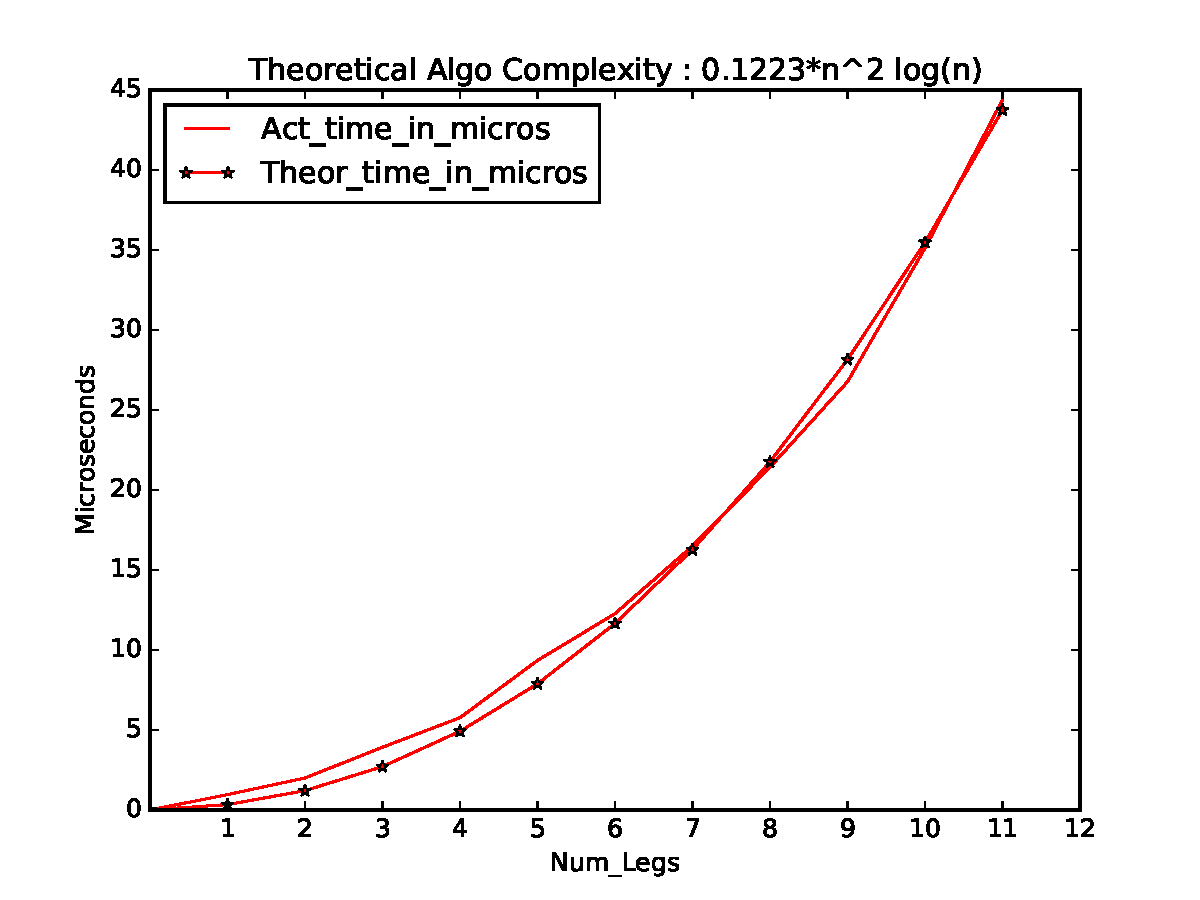
\includegraphics[scale=.55]{algo_complexity.pdf}
\caption{Algorighm running time with theoretical fit}
\end{figure}

We also can calculate the update time (time start: immediately after incoming quote is parsed, time end: full update of quote objects and task returns success; exactly the 4 steps above).  The following tables show times for a single update step on a single EC2 RedHat m2.large node:



a 4-core CentOS linux commodity machine. Times are in microseconds. Note that this time includes an update of the user quote object with the incoming quote, a step that would have to be performed in any case whether we were computing implied prices or not.

Benchmark tests were run on a 2.3GHz Intel Xeon E5-2686 v4 Broadwell, 4-core machine with 16Gb RAM.
 
\clearpage
\begin{table}
\centering
\begin{tabular}{|l|c|c|c|c|c|}
\hline
N & Average & Min & Max & Stddev & Num \\
\hline
0 & 14.563158 & 11 & 31 & 3.567040 & 9500 \\ 
1 & 14.295474 & 11 & 30 & 3.323515 & 9500 \\ 
2 & 14.150211 & 11 & 29 & 3.369054 & 9500 \\ 
3 & 14.012737 & 11 & 28 & 2.926719 & 9500 \\ 
4 & 14.050211 & 11 & 29 & 3.124248 & 9500 \\ 
5 & 13.997158 & 11 & 28 & 3.082419 & 9500 \\ 
6 & 13.974526 & 11 & 27 & 2.821791 & 9500 \\ 
7 & 14.220842 & 11 & 29 & 3.148978 & 9500 \\ 
8 & 13.908105 & 11 & 27 & 2.767451 & 9500 \\ 
9 & 13.945158 & 11 & 27 & 2.911735 & 9500 \\ 
\hline
\end{tabular}
\caption{12-Leg Problem, 10 Iterations}
\label{tab:template}
\end{table}

\begin{table}
\centering
\begin{tabular}{|l|c|c|c|c|c|}
\hline
N & Average & Min & Max & Stddev & Num \\
\hline
0 & 11.265895 & 8 & 26 & 3.154317 & 9500 \\ 
1 & 10.876737 & 8 & 24 & 2.717391 & 9500 \\ 
2 & 10.807263 & 8 & 23 & 2.611048 & 9500 \\ 
3 & 10.714737 & 8 & 23 & 2.612919 & 9500 \\ 
4 & 10.792737 & 8 & 23 & 2.466470 & 9500 \\ 
5 & 10.839158 & 8 & 23 & 2.601639 & 9500 \\ 
6 & 10.902632 & 8 & 24 & 2.816397 & 9500 \\ 
7 & 10.886947 & 8 & 25 & 2.793006 & 9500 \\ 
8 & 10.790632 & 8 & 23 & 2.615368 & 9500 \\ 
9 & 10.914737 & 8 & 24 & 2.721616 & 9500 \\ 
\hline
\end{tabular}
\caption{11-Leg Problem, 10 Iterations}
\label{tab:template}
\end{table}

\begin{table}
\centering
\begin{tabular}{|l|c|c|c|c|c|}
\hline
N & Average & Min & Max & Stddev & Num \\
\hline
0 & 10.218000 & 8 & 25 & 2.835815 & 9500 \\ 
1 & 9.975474 & 8 & 23 & 2.480480 & 9500 \\ 
2 & 9.948947 & 8 & 24 & 2.475615 & 9500 \\ 
3 & 9.834000 & 8 & 22 & 2.142498 & 9500 \\ 
4 & 10.079263 & 8 & 24 & 2.683880 & 9500 \\ 
5 & 9.976737 & 8 & 24 & 2.604584 & 9500 \\ 
6 & 10.039368 & 8 & 22 & 2.475212 & 9500 \\ 
7 & 9.976737 & 8 & 22 & 2.221967 & 9500 \\ 
8 & 9.970211 & 8 & 23 & 2.303404 & 9500 \\ 
9 & 9.810105 & 8 & 22 & 2.097212 & 9500 \\ 
\hline
\end{tabular}
\caption{10-Leg Problem, 10 Iterations}
\label{tab:template}
\end{table}

\begin{table}
\centering
\begin{tabular}{|l|c|c|c|c|c|}
\hline
N & Average & Min & Max & Stddev & Num \\
\hline
0 & 8.095368 & 6 & 20 & 1.988481 & 9500 \\ 
1 & 8.238316 & 6 & 18 & 2.100899 & 9500 \\ 
2 & 8.033263 & 6 & 20 & 1.907523 & 9500 \\ 
3 & 8.079474 & 6 & 21 & 2.086936 & 9500 \\ 
4 & 7.972211 & 6 & 17 & 1.614646 & 9500 \\ 
5 & 7.932211 & 6 & 18 & 1.664525 & 9500 \\ 
6 & 8.004211 & 6 & 20 & 1.844572 & 9500 \\ 
7 & 8.142632 & 6 & 21 & 2.089525 & 9500 \\ 
8 & 8.077263 & 6 & 21 & 2.061618 & 9500 \\ 
9 & 8.084421 & 6 & 20 & 2.041992 & 9500 \\ 
\hline
\end{tabular}
\caption{9-Leg Problem, 10 Iterations}
\label{tab:template}
\end{table}

\begin{table}
\centering
\begin{tabular}{|l|c|c|c|c|c|}
\hline
N & Average & Min & Max & Stddev & Num \\
\hline
0 & 6.198421 & 5 & 15 & 1.519532 & 9500 \\ 
1 & 6.165895 & 5 & 15 & 1.528084 & 9500 \\ 
2 & 6.145053 & 5 & 17 & 1.666477 & 9500 \\ 
3 & 6.159158 & 5 & 15 & 1.467598 & 9500 \\ 
4 & 6.061684 & 5 & 15 & 1.484377 & 9500 \\ 
5 & 6.272000 & 5 & 17 & 1.800889 & 9500 \\ 
6 & 6.078842 & 5 & 16 & 1.576353 & 9500 \\ 
7 & 6.072632 & 5 & 16 & 1.454141 & 9500 \\ 
8 & 6.256316 & 5 & 15 & 1.591008 & 9500 \\ 
9 & 6.163158 & 5 & 15 & 1.569364 & 9500 \\
\hline
\end{tabular}
\caption{8-Leg Problem, 10 Iterations}
\label{tab:template}
\end{table}

\begin{table}
\centering
\begin{tabular}{|l|c|c|c|c|c|}
\hline
N & Average & Min & Max & Stddev & Num \\
\hline
0 & 4.422737 & 3 & 12 & 1.067384 & 9500 \\ 
1 & 4.415579 & 3 & 12 & 1.096525 & 9500 \\ 
2 & 4.411895 & 3 & 10 & 0.936406 & 9500 \\ 
3 & 4.397053 & 3 & 12 & 1.036156 & 9500 \\ 
4 & 4.316632 & 3 & 12 & 0.947155 & 9500 \\ 
5 & 4.356000 & 3 & 12 & 1.034819 & 9500 \\ 
6 & 4.353895 & 3 & 12 & 0.960325 & 9500 \\ 
7 & 4.664421 & 3 & 13 & 1.448348 & 9500 \\ 
8 & 4.301895 & 3 & 12 & 0.919325 & 9500 \\ 
9 & 4.434211 & 3 & 12 & 1.131518 & 9500 \\
\hline
\end{tabular}
\caption{7-Leg Problem, 10 Iterations}
\label{tab:template}
\end{table}

\begin{table}
\centering
\begin{tabular}{|l|c|c|c|c|c|}
\hline
N & Average & Min & Max & Stddev & Num \\
\hline
0 & 3.025474 & 2 & 7 & 0.816572 & 9500 \\ 
1 & 3.023053 & 2 & 7 & 0.795552 & 9500 \\ 
2 & 2.967789 & 2 & 7 & 0.788788 & 9500 \\ 
3 & 3.022316 & 2 & 7 & 0.803408 & 9500 \\ 
4 & 3.050737 & 2 & 7 & 0.852258 & 9500 \\ 
5 & 2.963895 & 2 & 7 & 0.751642 & 9500 \\ 
6 & 2.983474 & 2 & 7 & 0.791071 & 9500 \\ 
7 & 3.108421 & 2 & 8 & 0.966451 & 9500 \\ 
8 & 3.275158 & 2 & 8 & 1.100045 & 9500 \\ 
9 & 2.990526 & 2 & 7 & 0.799854 & 9500 \\
\hline
\end{tabular}
\caption{6-Leg Problem, 10 Iterations}
\label{tab:template}
\end{table}

\clearpage
\section*{Curve Evolution}

This is a typical snapshot of the user vs. implied price (no size) for a simulated data set. The simulator produces prices in legs and calendar spread contracts, maintaining no-arbitrage conditions across the curve, and producing realistic bid-ask spreads and shape throughout the curve. This snapshot represents the market at sequence number 1350.


The implied quote curve gives a more comprehensive, arguably better notion of fair value across the curve. Note that implied prices are narrower starting at about the second or third leg, matching experience in these markets.


A full evolution for a randomly selected interval of sequence numbers is given in the file {\it quote{\_}evolution.pdf}.

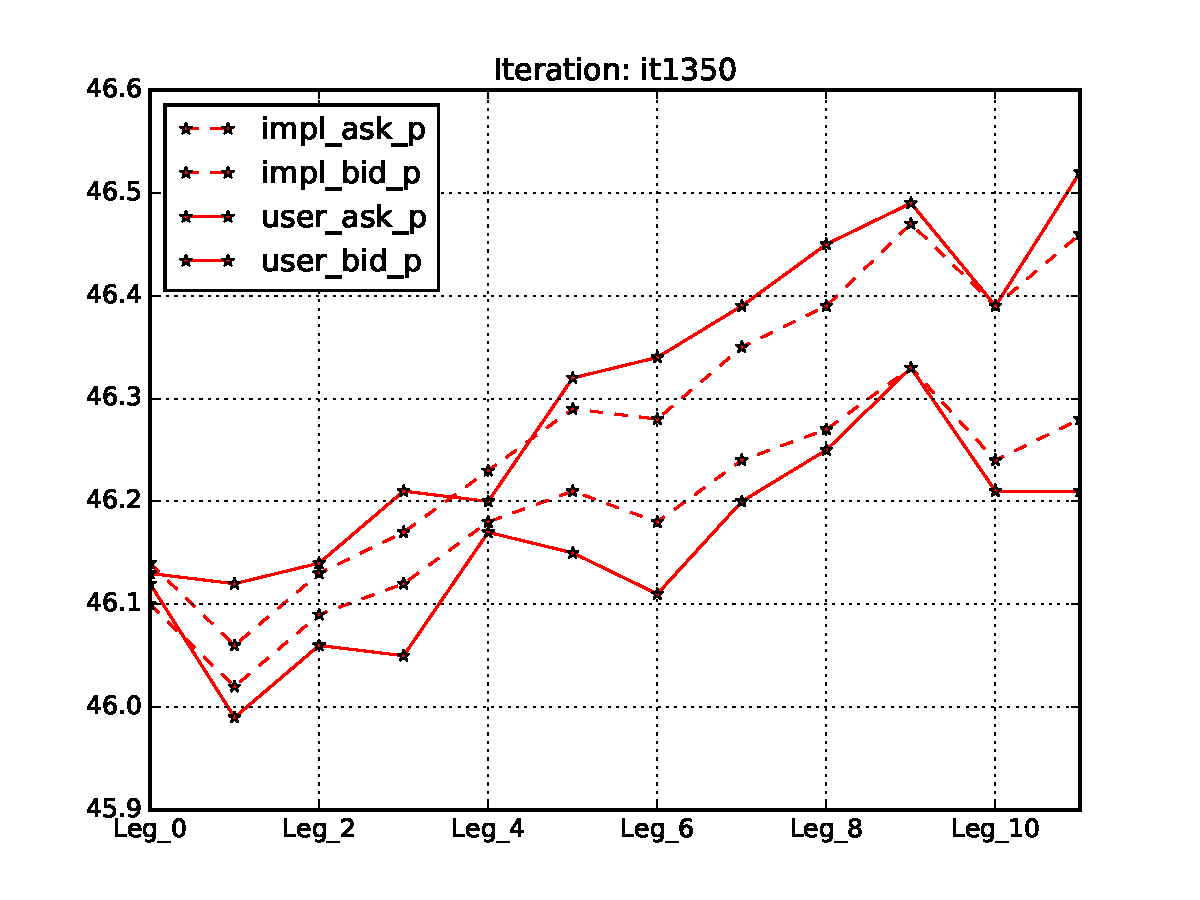
\includegraphics[scale=.75]{quote_comp.pdf}


\end{document}
